\documentclass[12pt, a4paper]{article}
\usepackage[utf8]{inputenc}
\usepackage[portuguese]{babel}
\usepackage[T1]{fontenc}
\usepackage{geometry}
\usepackage{amsmath}
\usepackage{amsfonts}
\usepackage{amssymb}
\usepackage{xcolor}
\usepackage{url}
\usepackage{hyperref}
\usepackage{setspace}
\usepackage{listings}
\usepackage{float}
\usepackage{graphicx}

\lstset{ 
    basicstyle=\ttfamily\small, % Fonte monoespaçada
    numbers=left, % Numeração das linhas
    numberstyle=\tiny\color{gray}, keywordstyle=\color{blue}, % Cor das palavras-chave
    commentstyle=\color{green!50!black}, % Cor dos comentários
    stringstyle=\color{red}, % Cor das strings
    breaklines=true, % Quebra automática de linha
    tabsize=2 % Tamanho do tab
}

% Configurações de página
\geometry{margin=2.5cm}
\onehalfspacing{}

% Configurações do hyperref
\hypersetup{
    colorlinks=true,
    linkcolor=black,
    filecolor=magenta,
    urlcolor=blue,
    citecolor=blue
}

\begin{document}
    \begin{titlepage}
        \centering
        \vspace*{2cm}

        {\huge\bfseries Projeto 2 --- DGEMM Sequencial e Paralela com MPI\par}
        \vspace{1.5cm}

        {\Large \textbf{Autores:}\\ Italo Santana Seara\\ Wilson Santos Silva Filho\\ }

        \vspace{2cm}

        {\large \textbf{Disciplina:} DEC107 — Processamento Paralelo\\ \textbf{Professor:} Esbel Tomas Valero Orellana\\ \textbf{Data:} \today\\ }

        \vfill
    \end{titlepage}

    \tableofcontents

    \newpage
    \section{Introdução}\label{sec:introducao}

    A multiplicação de matrizes é uma operação fundamental em diversas áreas da computação científica e engenharia, presente em aplicações que vão desde álgebra linear numérica até aprendizagem de máquina e simulações físicas. Neste projeto, focamos na versão de precisão dupla da multiplicação geral de matrizes (DGEMM), cujo problema pode ser formalizado como: dado $A\in\mathbb{R}^{m\times k}$ e $B\in\mathbb{R}^{k\times n}$, calcular $C=AB$, onde
    
    \[
        C_{ij}=\sum_{t=1}^{k} A_{it}\,B_{tj}, \qquad 1 \le i \le m, \;1 \le j \le n.
    \]

    A complexidade aritmética desta operação cresce como $\mathcal{O}(mkn)$ e, para matrizes quadradas de ordem $N$, como $\mathcal{O}(N^{3})$, o que torna essencial a exploração de paralelismo para resolver instâncias de grande porte de forma eficiente.

    No Projeto 1 foram implementadas versões sequenciais e paralelas (por memória compartilhada, com OpenMP) da DGEMM.\@ No presente Projeto 2, damos continuidade ao estudo do paralelismo ao migrar para o modelo de memória distribuída, implementando a DGEMM com o padrão MPI (Message Passing Interface). O objetivo central é projetar e avaliar uma implementação paralela distribuída que explore comunicação por troca de mensagens entre processos, comparando sua corretude e desempenho com as versões sequencial e com OpenMP.\@

    Este projeto tem como objetivos específicos:
    \begin{itemize}
        \item Implementar uma versão paralela distribuída de DGEMM utilizando apenas rotinas básicas do MPI (por exemplo, \texttt{MPI\_Init}, \texttt{MPI\_Comm\_size}, \texttt{MPI\_Comm\_rank}, \texttt{MPI\_Send}, \texttt{MPI\_Recv}, \texttt{MPI\_Bcast}, \texttt{MPI\_Scatter}, \texttt{MPI\_Gather}).
        \item Validar a corretude numérica da implementação MPI comparando-a com a versão sequencial e calculando a diferença relativa máxima entre os elementos do resultado, usando estratégias que evitem divisão por zero.
        \item Medir e analisar desempenho (tempo total, \emph{speedup} e eficiência) em várias configurações de processos e tamanhos de matrizes, e comparar os resultados com os obtidos em ambiente de memória compartilhada (OpenMP).
        \item Discutir trade-offs entre modelos de memória (compartilhada vs distribuída), identificando gargalos relacionados à comunicação (latência e largura de banda) e ao balanceamento de carga.
    \end{itemize}

    Para atingir esses objetivos, a estratégia adotada contempla a decomposição das matrizes por blocos (linhas ou colunas) --- detalhada na seção de metodologia --- e a utilização de vetores unidimensionais (\textit{C-style arrays}) para o armazenamento compacto das matrizes. A análise de desempenho considera tempos médios sobre múltiplas execuções e avalia tamanhos de problema representativos (por exemplo, ordens 512, 1024, 2048 e 4096), assim como configurações com 1, 2, 4 e, quando possível, 8 processos.

    Este relatório está organizado da seguinte forma: na Seção~\ref{sec:metodologia} descreve-se a implementação sequencial e paralela, as rotinas MPI utilizadas e a metodologia de medição; a Seção~\ref{sec:resultados} apresenta testes de corretude, tabelas e gráficos de desempenho e os cálculos de \emph{speedup} e eficiência; a Seção~\ref{sec:discussao} analisa os resultados e discute limitações; por fim, a Seção~\ref{sec:conclusao} sintetiza os aprendizados e sugere melhorias futuras.

    \newpage
    \section{Metodologia}\label{sec:metodologia}

    Nesta seção, detalhamos a implementação da multiplicação de matrizes DGEMM em suas versões sequencial e paralela utilizando MPI, bem como a metodologia adotada para medir desempenho e validar corretude.

    \subsection{Implementação Sequencial}

    A implementação sequencial da DGEMM utiliza a versão otimizada do Projeto 1, que emprega blocos para melhorar a localidade de dados. As matrizes são armazenadas em vetores unidimensionais (\textit{C-style arrays}) para garantir um acesso eficiente à memória. A função principal responsável pela multiplicação é apresentada no repositório do projeto.\footnotemark[1]

    Esta implementação serve como referência para comparação de desempenho com a versão paralela.

    \subsection{Implementação Paralela com OpenMP}

    A versão paralela com OpenMP, desenvolvida no Projeto 1, utiliza diretivas de paralelismo para distribuir o trabalho entre múltiplas threads em um ambiente de memória compartilhada. A decomposição por blocos é mantida, e a paralelização é aplicada principalmente nos loops externos da multiplicação de matrizes. 
    
    Esta implementação também está disponível no repositório do projeto.\footnotemark[1]

    \subsection{Implementação Paralela com MPI}

    A versão paralela da DGEMM foi desenvolvida utilizando o padrão MPI, que permite a comunicação entre processos em um ambiente de memória distribuída. A estratégia adotada envolve a decomposição das matrizes por blocos, onde cada processo é responsável por calcular uma parte da matriz resultado $C$. A seguir, descrevemos os principais passos da implementação:
    
    \begin{itemize}
        \item Inicialização do ambiente MPI utilizando \texttt{MPI\_Init}.
        \item Determinação do número total de processos e do identificador de cada processo com \texttt{MPI\_Comm\_size} e \texttt{MPI\_Comm\_rank}.
        \item Distribuição das matrizes $A$ e $B$ entre os processos utilizando \texttt{MPI\_Scatter} para $A$ e \texttt{MPI\_Bcast} para $B$.
        \item Cada processo calcula sua parte da matriz $C$ localmente.
        \item Coleta dos resultados parciais de $C$ utilizando \texttt{MPI\_Gather} (apenas o processo raiz (rank 0) retorna o resultado final).
        \item Finalização do ambiente MPI com \texttt{MPI\_Finalize}.
    \end{itemize}

    A implementação completa está disponível no repositório do projeto.\footnotemark[1]

    \footnotetext[1]{Link para as implementações: \url{https://github.com/italoseara/DEC107/blob/main/Projeto 2/src/dgemm.c}}

    \subsection{Validação de Corretude}

    A corretude da implementação sequencial e com OpenMP não foram validadas no relatório do Projeto 1, portanto, desta vez, a versão sequencial foi validada comparando os resultados obtidos com a função \texttt{cblas\_dgemm} da biblioteca BLAS (Basic Linear Algebra Subprograms), que é amplamente reconhecida por sua eficiência e precisão numérica. A versão com OpenMP foi validada comparando seus resultados com os da versão sequencial, da mesma forma que a versão MPI.\@

    A corretude da implementação paralela com MPI foi realizada comparando o resultado obtido com o da versão sequencial, calculando a diferença relativa máxima entre os elementos das matrizes resultantes, utilizando uma abordagem que evita divisão por zero. A fórmula utilizada foi:

    \[
        \Delta = \max_{i,j} \frac{|C_{\text{seq}}(i, j) - C_{\text{mpi}}(i, j)|}{|C_{\text{seq}}(i, j)| + \epsilon}, \quad \epsilon = 10^{-12}
    \]

    Considerando corretas implementações cuja diferença relativa máxima seja inferior a $10^{-9}$.

    \subsection{Descrição do hardware utilizado nos testes}

    Os testes foram realizados em uma máquina com as seguintes especificações:
    \begin{itemize}
        \item \textbf{Processador:} Ryzen 7 5700G (8 núcleos)
        \item \textbf{Memória RAM:} 32 GB
        \item \textbf{Sistema Operacional:} Windows 11 + WSL 2.4.10.0 (Ubuntu 24.04.2 LTS)
        \item \textbf{Compilador:} GCC 13.3.0
    \end{itemize}

    \subsection{Métricas utilizadas para avaliação}
	
    Usaremos as seguintes métricas para definir e comparar as implementações:

    \subsubsection{Tempo de Execução}

    Medido em segundos, é o tempo total gasto para completar a multiplicação das matrizes. Não inclui o tempo de inicialização ou finalização do programa, apenas o tempo gasto na execução da função de multiplicação.
    \[
        T = T_{end} - T_{start}
    \]
    Onde:
    \begin{itemize}
        \item $T$ é o tempo de execução.
        \item $T_{start}$ é o tempo registrado no início da execução da função.
        \item $T_{end}$ é o tempo registrado ao final da execução da função.
    \end{itemize}

    O tempo total de execução será medido utilizando a função \texttt{MPI\_Wtime()} para a versão MPI, e \texttt{omp\_get\_wtime()} para a versão OpenMP e para a versão sequencial.

    Foi utilizado um script em python para automatizar a execução dos testes e coletar os tempos. O script executa cada versão múltiplas vezes com diferentes entradas para obter uma média dos tempos, calcula as métricas de desempenho e gera um relatório com os resultados, que foram utilizados para criar os gráficos apresentados na seção de resultados.

    \subsubsection{Speedup}
	Mede o ganho de desempenho da versão paralela em relação à sequencial.
	\[
		S_{p} = \frac{T_{s}}{T_{p}}
	\]
	Onde:
	\begin{itemize}
		\item $S_{p}$ é o speedup com $p$ processadores/threads.

		\item $T_{s}$ é o tempo de execução da versão sequencial.

		\item $T_{p}$ é o tempo de execução da versão paralela com $p$ processadores/threads.
	\end{itemize}

	\subsubsection{Eficiência}
    Mede quão bem os recursos de processamento estão sendo utilizados pela versão paralela. Onde 1 é a eficiência ideal (100\%).
	\[
		E_{p} = \frac{S_{p}}{p}= \frac{T_{s}}{p \cdot T_{p}}
	\]
	Onde:
	\begin{itemize}
		\item $E_{p}$ é a eficiência com $p$ processadores/threads. Varia entre 0 e 1.

		\item $S_{p}$ é o speedup com $p$ processadores/threads.

        \item $p$ é o número de processadores/threads.

        \item $T_{s}$ é o tempo de execução da versão sequencial.

        \item $T_{p}$ é o tempo de execução da versão paralela com $p$ processadores/threads.
	\end{itemize}

    \newpage
    \section{Resultados}\label{sec:resultados}

    Nesta seção, apresentamos os resultados obtidos a partir dos testes realizados nas implementações sequencial, paralela com OpenMP e paralela com MPI da multiplicação de matrizes DGEMM.\@ Os resultados incluem a validação de corretude, tabelas e gráficos de desempenho, bem como cálculos de \emph{speedup} e eficiência.

    Uma diferença em relação ao Projeto 1 é que o \emph{speedup} e a eficiência foram calculados em relação à mesma implementação porém com 1 thread/processo, ou seja, a implementação com OpenMP foi comparada com ela mesma utilizando 1 thread, e a implementação com MPI foi comparada com ela mesma utilizando 1 processo. Isso foi feito para evitar que diferenças de implementação afetassem os resultados de \emph{speedup} e eficiência.

    \subsection{Tempo de execução}

    \begin{figure}[H]
        \centering
        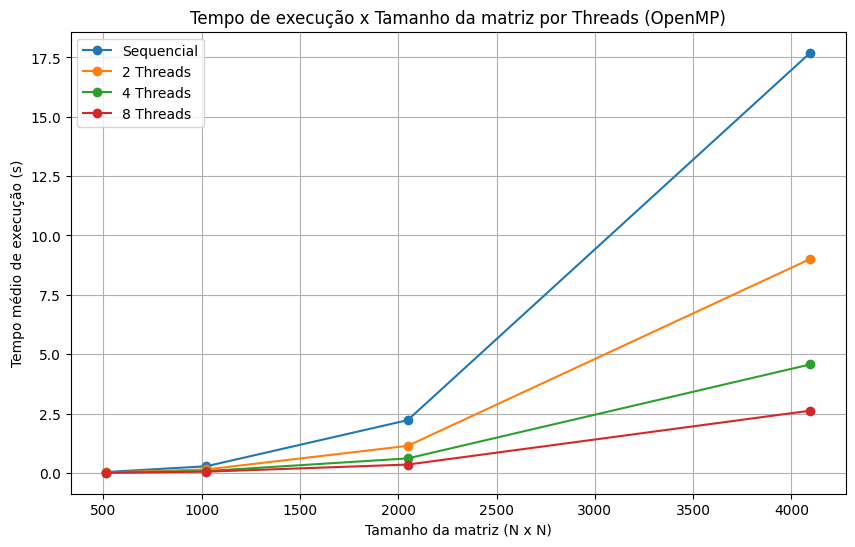
\includegraphics[width=0.9\textwidth]{img/execution-time-openmp.png}
        \caption{Tempo de execução (OpenMP)}\label{fig:tempo_execucao_omp}
    \end{figure}

    \begin{figure}[H]
        \centering
        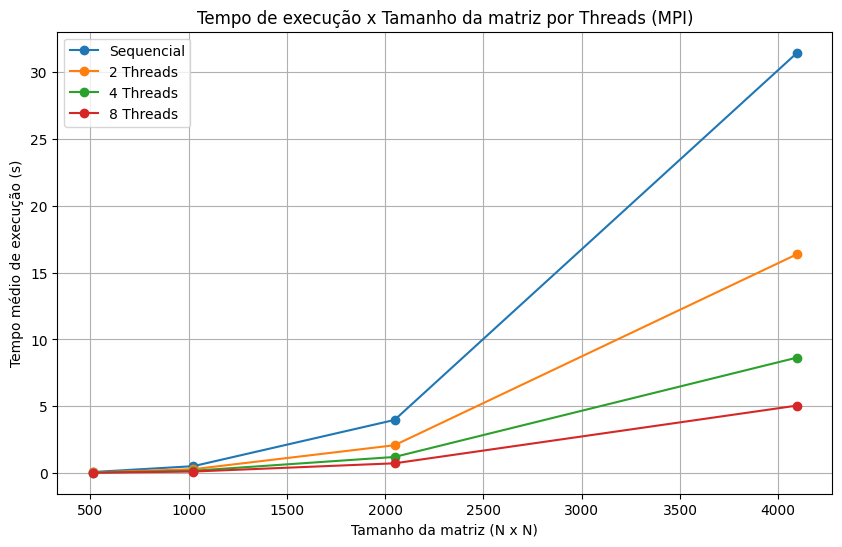
\includegraphics[width=0.9\textwidth]{img/execution-time-mpi.png}
        \caption{Tempo de execução (MPI)}\label{fig:tempo_execucao_mpi}
    \end{figure}

    As Figuras~\ref{fig:tempo_execucao_omp} e~\ref{fig:tempo_execucao_mpi} mostram o tempo de execução das implementações com OpenMP e MPI, respectivamente, para diferentes tamanhos de matrizes e números de threads/processos. Observa-se que o tempo de execução diminui com o aumento do número de threads/processos, evidenciando o benefício do paralelismo. Contudo, é possível perceber que a implementação com OpenMP apresenta tempos de execução menores em comparação com a implementação com MPI para o mesmo número de threads/processos, o que pode ser atribuído à sobrecarga de comunicação inerente ao modelo de memória distribuída utilizado pelo MPI.\@

    \subsection{Speedup}

    \begin{figure}[H]
        \centering
        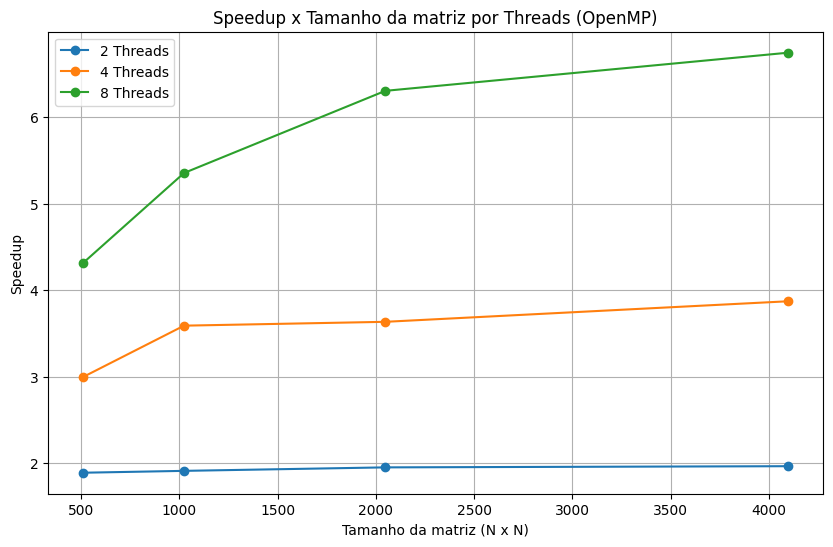
\includegraphics[width=0.9\textwidth]{img/speedup-openmp.png}
        \caption{Speedup (OpenMP)}\label{fig:speedup_omp}
    \end{figure}

    \begin{figure}[H]
        \centering
        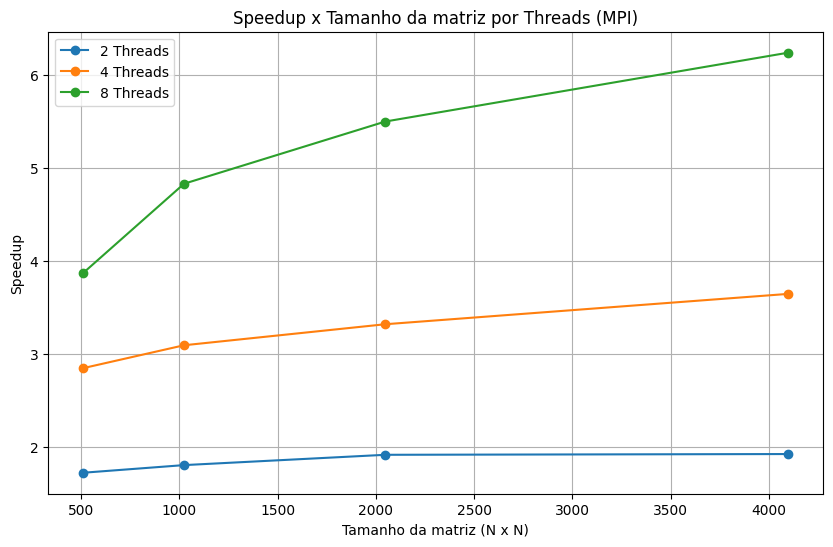
\includegraphics[width=0.9\textwidth]{img/speedup-mpi.png}
        \caption{Speedup (MPI)}\label{fig:speedup_mpi}
    \end{figure}

    As Figuras~\ref{fig:speedup_omp} e~\ref{fig:speedup_mpi} apresentam o \emph{speedup} obtido pelas implementações com OpenMP e MPI, respectivamente. Observa-se que ambas as implementações conseguem alcançar um \emph{speedup} significativo com o aumento do número de threads/processos.

    \subsection{Eficiência}

    \begin{figure}[H]
        \centering
        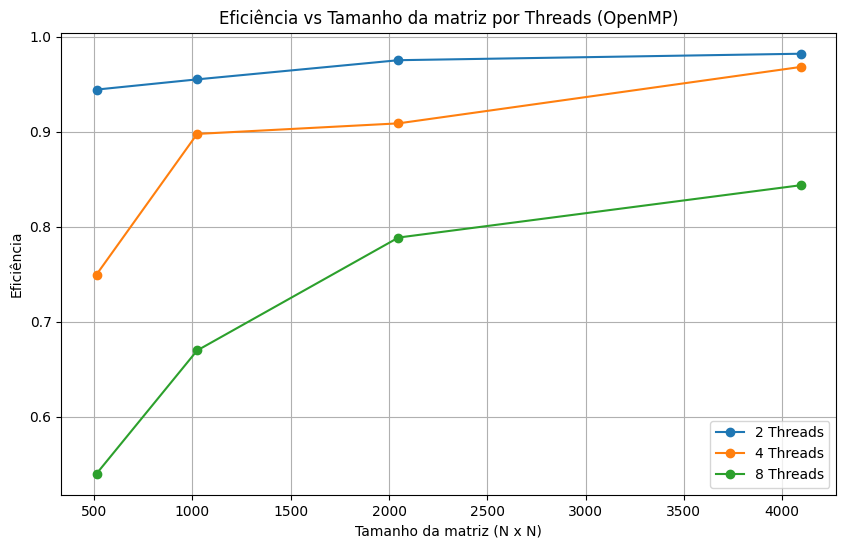
\includegraphics[width=0.9\textwidth]{img/efficiency-openmp.png}
        \caption{Eficiência (OpenMP)}\label{fig:eficiencia_omp}
    \end{figure}

    \begin{figure}[H]
        \centering
        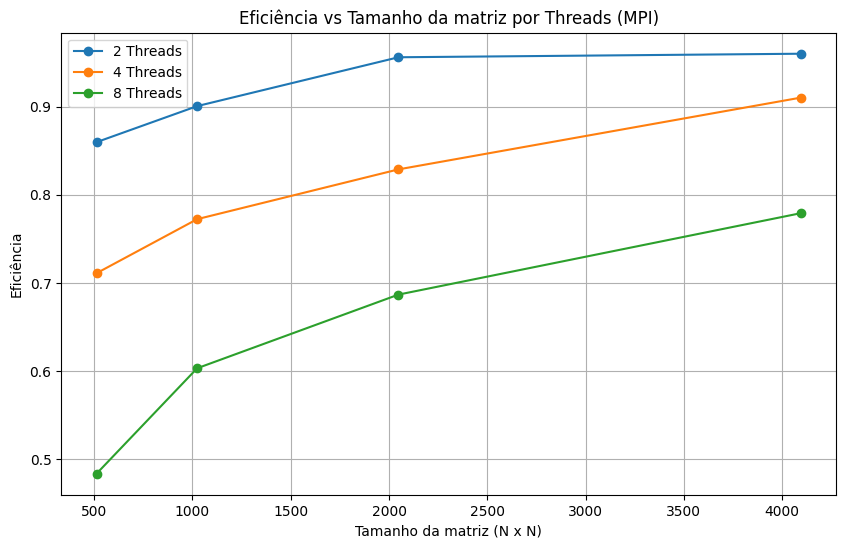
\includegraphics[width=0.9\textwidth]{img/efficiency-mpi.png}
        \caption{Eficiência (MPI)}\label{fig:eficiencia_mpi}
    \end{figure}

    As Figuras~\ref{fig:eficiencia_omp} e~\ref{fig:eficiencia_mpi} mostram a eficiência das implementações com OpenMP e MPI, respectivamente. A eficiência tende a diminuir com o aumento do número de threads/processos, o que é esperado devido à sobrecarga de comunicação e sincronização. Não há uma diferença significativa na eficiência entre as duas implementações, embora a implementação com OpenMP apresente uma leve vantagem em alguns casos.

    \newpage
    \section{Discussão}\label{sec:discussao}

    Nesta seção, discutimos os resultados obtidos nas implementações sequencial, paralela com OpenMP e paralela com MPI da multiplicação de matrizes DGEMM.\@ Analisamos o desempenho, a escalabilidade e as limitações de cada abordagem.

    \subsection{Análise de Desempenho}

    A implementação com OpenMP apresentou um desempenho superior em comparação com a implementação com MPI para o mesmo número de threads/processos. Isso pode ser atribuído à menor sobrecarga de comunicação no modelo de memória compartilhada utilizado pelo OpenMP, em contraste com o modelo de memória distribuída do MPI, que requer troca de mensagens entre processos.

    \subsection{Escalabilidade}

    Ambas as implementações demonstraram boa escalabilidade com o aumento do número de threads/processos. No entanto, a eficiência diminuiu à medida que o número de threads/processos aumentou, indicando que a sobrecarga de comunicação e sincronização começa a impactar negativamente o desempenho em configurações com muitos processos.

    Porém, a versão com MPI possui uma vantagem clara: sua capacidade de escalar para um número maior de processos em ambientes distribuídos, como clusters de computadores, onde o OpenMP não é aplicável. Isso torna a implementação com MPI mais adequada para aplicações que exigem alta escalabilidade e distribuição de carga em múltiplos nós.

    \subsection{Limitações}

    Uma limitação observada na implementação com MPI é a complexidade adicional na gestão da comunicação entre processos, o que levou a diversos erros e dificuldades no debug. Além disso, a sobrecarga de comunicação pode se tornar um gargalo em sistemas com alta latência ou largura de banda limitada.

    \newpage
    \section{Conclusão}\label{sec:conclusao}

    Neste relatório, apresentamos a implementação e análise de desempenho da multiplicação de matrizes DGEMM em suas versões sequencial, paralela com OpenMP e paralela com MPI.A implementação com OpenMP demonstrou um desempenho superior em ambientes de memória compartilhada, enquanto a implementação com MPI destacou-se pela sua capacidade de escalar em ambientes distribuídos. Ambas as implementações apresentaram boa escalabilidade, embora a eficiência tenha diminuído com o aumento do número de threads/processos devido à sobrecarga de comunicação.

    Em trabalhos futuros, sugerimos explorar otimizações adicionais na implementação com MPI, como o uso de técnicas avançadas de comunicação e balanceamento de carga. Além disso, seria interessante investigar a combinação de OpenMP e MPI para aproveitar os benefícios de ambos os modelos de paralelismo em sistemas híbridos.

    \newpage
    \begin{thebibliography}{9}
    \raggedright{}
        \bibitem{latexcompanion} Orellana, E., \texttt{Materiais de slides vistos em aula}

        \bibitem{latexcompanion} OPENMP, Disponível em: \url{https://www.openmp.org/wp-content/uploads/OpenMP-RefGuide-6.0-OMP60SC24-web.pdf}. Acesso em: 22 de Setembro de 2025.

        \bibitem{knuthwebsite} Brasil Escola, Disponível em: \url{https://brasilescola.uol.com.br/matematica/multiplicacao-matrizes.htm}. Acesso em: 22 de Setembro de 2025.

        \bibitem{knuthwebsite} VSP-BERLIN, Disponível em: \url{https://svn.vsp.tu-berlin.de/repos/public-svn/publications/kn-old/strc/html/node9.html}. Acesso em: 23 de Setembro de 2025.

        \bibitem{knuthwebsite} Wikipedia, Disponível em: \url{https://en.wikipedia.org/wiki/Loop\_nest\_optimization}. Acesso em: 23 de Setembro de 2025.
    \end{thebibliography}

\end{document}
